% Documento LaTeX
% Tipo de documento y tamaño de letra
\documentclass[10pt]{article}
% Preparando para documento en Español.
% Para documento en Inglés no hay que hacer esto.
\usepackage[spanish]{babel}
\selectlanguage{spanish}
\usepackage[utf8]{inputenc}
\usepackage{graphicx}
% EL titulo, autor y fecha del documento
\title{Iniciando con FORTRAN}
\author{Luisa Fernanda Orci Fernandez.}
\date{17 de Febrero del 2015}
% Aqui comienza el cuerpo del documento
\begin{document}
% Construye el título
\maketitle
\section{Introducción}
Esta actividad está conformada por una serie de ejercicios breves en Fortran, que nos sirven para calcular áreas, volumenes, así como algunos ejemplos de como resolver funciones.\\

\section{Calcular el área de un circulo.}
Con este programa se puede calcular facilmente el área de un circulo. El programa está diseñado para que el usuario de un radio y a partir de eso dar el resultado del área.\\
A continuación, el código utilizado para calcular el área, seguido del resultado al compilarlo.
\begin{verbatim}
! Area . f90 : Calculates the area of a circle, sample program
! -----------------------------------------------

Program Circle_area ! Begin main program
  Implicit None ! Declare all variables
  Real *8 :: radius , circum , area ! Declare reals
  Real *8 :: PI= 4.0 * atan(1.0) ! Declare, assing Real
  Integer :: model_n = 1 ! Declare, assing Ints
  print *, 'Enter a radius:' ! Talk to user
  read *, radius ! Read into radius
  circum = 2.0 * PI * radius ! Calc circumference
  area = radius * radius * PI ! Calc area
  print * , 'Program number = ' , model_n ! Print program number
  print * , 'Radius =' , radius ! Print radius
  print * , 'Circumference =' , circum ! Print circumference
  print * , 'Area=' , area ! Print area
 
End Program Circle_area ! End main program code
\end{verbatim}
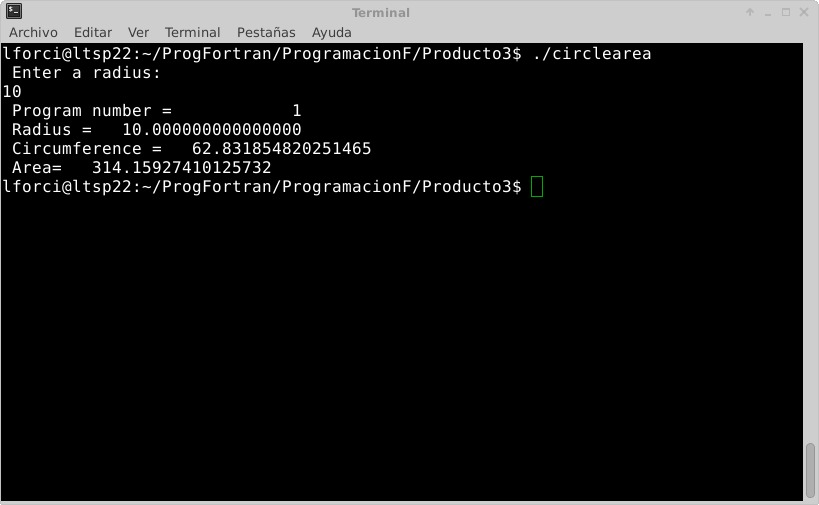
\includegraphics[scale=0.6]{CircleArea}

\section{Calcular el volumen de un tanque esférico de radio r y altura h.}
Este programa sirve para calcular el volumen de un tanque que no está completamente lleno. Al usuario se le pide que proporcione un radio y la altura hasta donde está lleno el tanque.\\
A continuación, el código utilizado para calcular el volumen, seguido del resultado al compilarlo.

\begin{verbatim}
  ! Volumen.f90: Calculates a spherical cap
  !------------------------------------

Program Volumen
  Implicit None
  ! Declarar mis variables, NO CALCULAR NADA
  Real *8 :: radio, circum, PI, vol, h
  Integer :: model_n = 2
  
  
  ! EPEZAR A realizar calculos y demas
  PI= 4.0 * atan(1.0)
  print *, 'Dame un radio'
  read *, radio
  print *, 'Dame una altura'
  read *, h
  circum= 2.0 * PI * radio
  vol= (PI*(h*h))*(radio-(h/3))
  print * , 'Program number = ' , model_n
  print *, 'Radio =' , radio
  print *, 'Altura=' , h
  print *, 'Circunferencia =' , circum
  print *, 'Volumen =' , vol
  
  
End 
\end{verbatim}
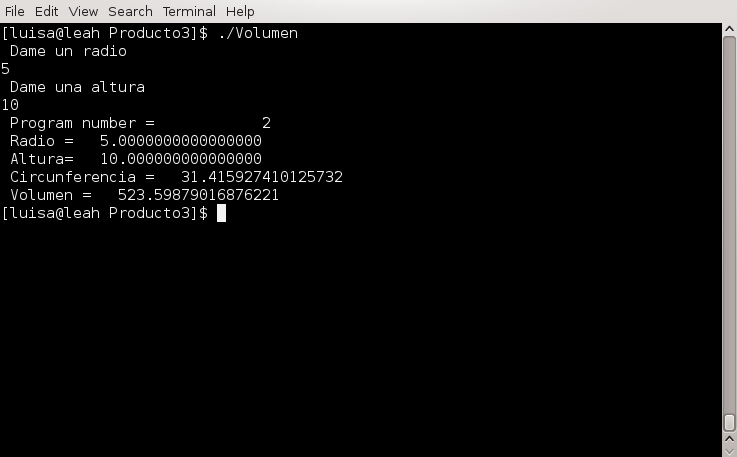
\includegraphics[scale=0.6]{Volumen}

\section{Determinar la precisión de la máquina.}
Este programa sirve para determinar la presición de la máquina.\\
A continuación, el código y un ejemplo de lo que sucede al compilar.
\begin{verbatim}
! Limits . f90: Determines machine precision
! -------------------------------

Program Limits
  Implicit None
  Integer :: i , n
  Real *4 :: epsilon_m , one
  n=60                        ! Establish the number of iterations
  ! Set Initial values:
  epsilon_m = 1.0
  one = 1.0
  ! Within a DO-LOOP, calculate each step and print.
  ! This loop will execute 60 times in a row as i is
  !   incremented from 1 to n (since n = 60):
  do i = 1, n, 1                  ! Begin the do-loop
     epsilon_m = epsilon_m / 2.0  ! Reduce epsilon_m
     one = 1.0 + epsilon_m        ! Re-calculate one
     print *, i, one, epsilon_m   ! Print values so far
     end do                       ! End loop when i>n

End program Limits

\end{verbatim}
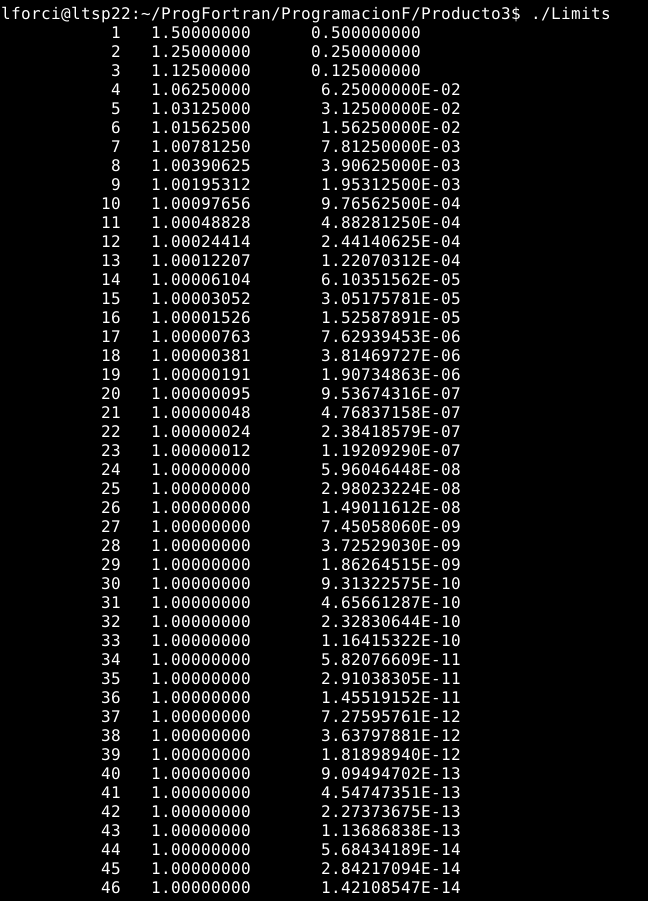
\includegraphics[scale=0.6]{Limits}

\section{Funciones matemáticas especiales.}
Fortran maneja las funciones especiales y las trigonométricas, pero no maneja la relación entre ellas.\\
A continuación un ejemplo para calcular la raíz cuadrada de -1, el arcoseno de 2 y el log10 de 0.

\begin{verbatim}
! Math . f90: demo some Fortran math functions
! --------------------------------------------

Program Math_test             ! Begin main program
  Real *8 :: x=-1.0, y=2.0, z=0    ! Declare variables x, y, z
  v = SQRT (x)                ! Call the Square root  function
  w = ASIN (y)                ! Call the Arcsine function
  f = LOG10 (z)               ! Call the Common logarithm function
  print *, v, w, f            ! Print x, y, z
 
End Program Math_test         ! End main program
\end{verbatim}
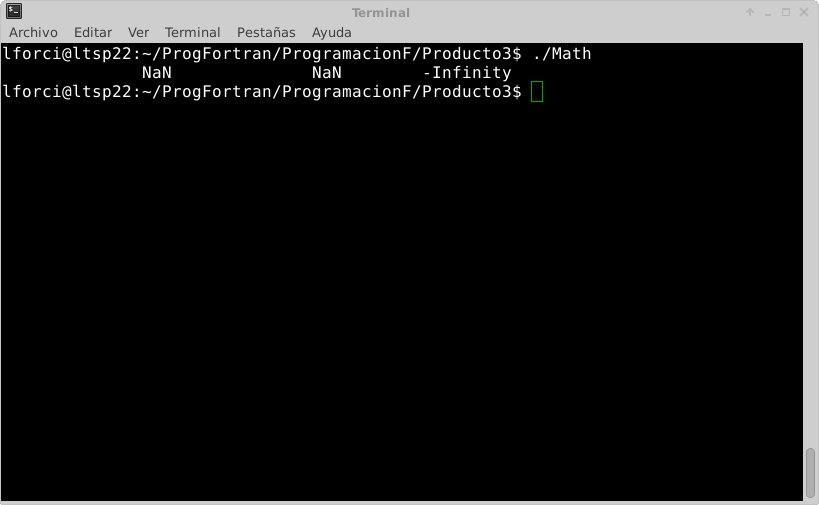
\includegraphics[scale=0.6]{Math}

\section{Calcular Funciones.}
En Fortran también nos sirve para calcular funciones.\\
A continuación un ejemplo de como calcular la funcion f(x)= 1+ sin(x y).
\begin{verbatim}
! Function . f90: Program calls a simple function
! ----------------------------------

Real*8 Function f(x,y)
  Implicit None
  Real*8 :: x, y
  f = 1.0 + sin(x*y)
End Function f

!

Program Main
  Implicit None
  Real*8 :: Xin=0.25, Yin=2., c, f ! declarations (also f)
  c = f(Xin, Yin)
  write(*,*) 'f(Xin, Yin) = ' ,c

End program Main
\end{verbatim}
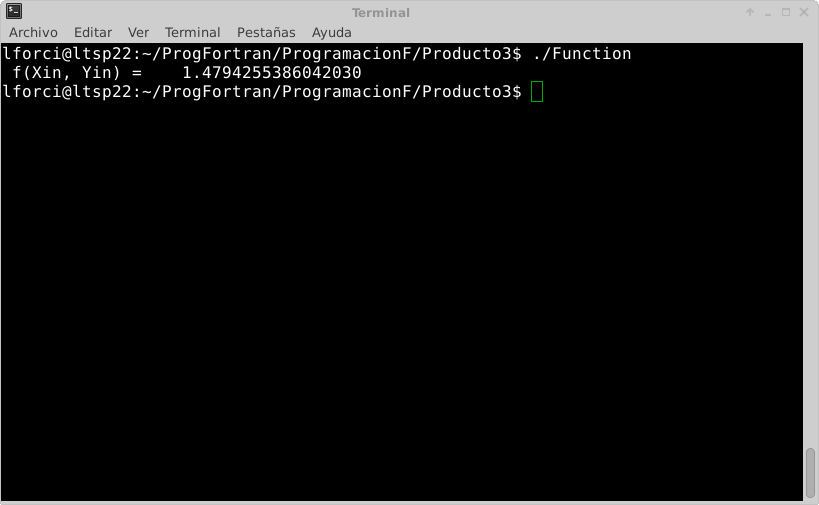
\includegraphics[scale=0.6]{Function}

\section{Subrutinas.}
En Fortran también podemos manejar subrutinas, estas sirven para encapsular y reutilizar funciones específicas.\\
A continuación un programa que contiene un ejemplo de subrutina.
\begin{verbatim}
! Subroutine . f90: Demonstrates the call for a simple subroutine
! ------------------------------------------------
Subroutine g(x, y, ans1, ans2)
  Implicit None
  Real(8) :: x, y, ans1, ans2 ! Declare variables
  ans1= sin(x*y) + 1.         ! Use sine intrinsic func.
  ans2= ans1**2
End Subroutine g

!

Program Main_program          ! Demos the CALL
  Implicit None
  Real *8 :: Xin=0.25, Yin=2.0, Gout1, Gout2
  call g(Xin, Yin, Gout1, Gout2) ! Call the subr g
  write (*, *) 'The answers are: ' , Gout1, Gout2

End Program Main_Program

\end{verbatim}
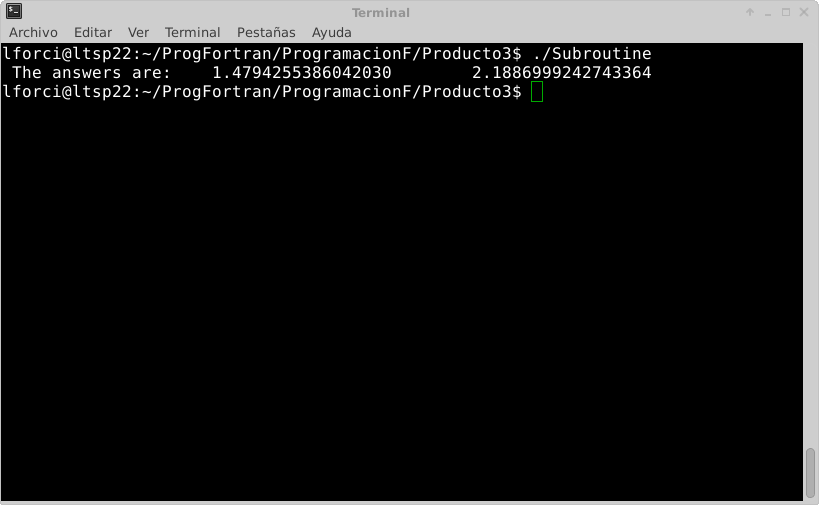
\includegraphics[scale=0.6]{Subroutine}

\end{document}
